\pagebreak
\section{Inertia Test}
\nopagebreak
%\subsection{} %\label{put a label here and uncomment}
\textbf{Name: Group 510}\\
\textbf{Date: 02/11 - 2015}

\subsubsection{Purpose}
The purpose of the test is to measure the inertia of the loaded vehicle $J_{tot}$.

\subsubsection{Setup}
\begin{figure}[H]
	\centering
	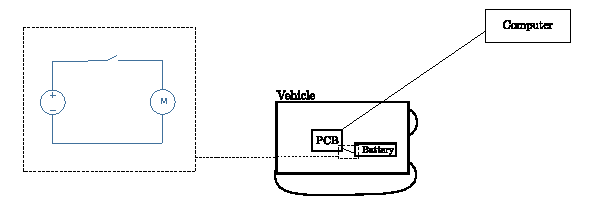
\includegraphics[scale=1.6]{figures/inertiaTestSetupDiagram.pdf}
	\caption{Setup diagram}
	\label{inertiaTestSetupDiagram}
\end{figure}

\subsubsection{List of Equipment}

\begin{table}[H]
\begin{tabular}{|p{10cm}|p{4cm}|}
\hline%------------------------------------------------------------------------------------
  \textbf{Instrument}                     &  \textbf{Type}       \\
\hline%------------------------------------------------------------------------------------
  Computer                                &  Asus N73JN    \\
\hline %-----------------------------------------------------------------------------------
\end{tabular}
\end{table}


\subsubsection{Procedure}

\begin{enumerate}
  \item Connect the vehicle to the computer via the arduino card, and disconnect the battery.
  \item Launch the arduino program.
  \item Plug in the battery so the vehicle runs.
  \item After a few seconds of running, take off the two wires connected to the PCB to stop powering the vehicle.
  \item Wait until the vehicle stops to end measuring the speed of it.
  \item Plot the speed of the vehicle.
\end{enumerate}

\subsubsection{Results}

\begin{figure}[H]
  \centering
  %\includegraphics[scale=0,5]{figures/InertiaTestPlot.pdf}
  \caption{Plot of the inertia measured speed of the vehicle.}
  \label{intertiaTestPlot}
\end{figure}

During these measurements the motor is at constant speed until the end when it is unpluged.